\appendix

\section{Le programme et son utilisation}
L'exécutable du projet est disponible dans le dossier target/dist. Pour l'exécuter, il suffit d'ouvrir un prompt et de lancer: \textbf{java -jar simulation.jar}.

\subsection{Configuration et aide}
Pour afficher la liste des paramètres pouvant être donnés au programme, il suffit d'ouvrir un prompt et de lancer: \textbf{java -jar simulation.jar --aide}


\begin{figure}[h!t]
  \centering
    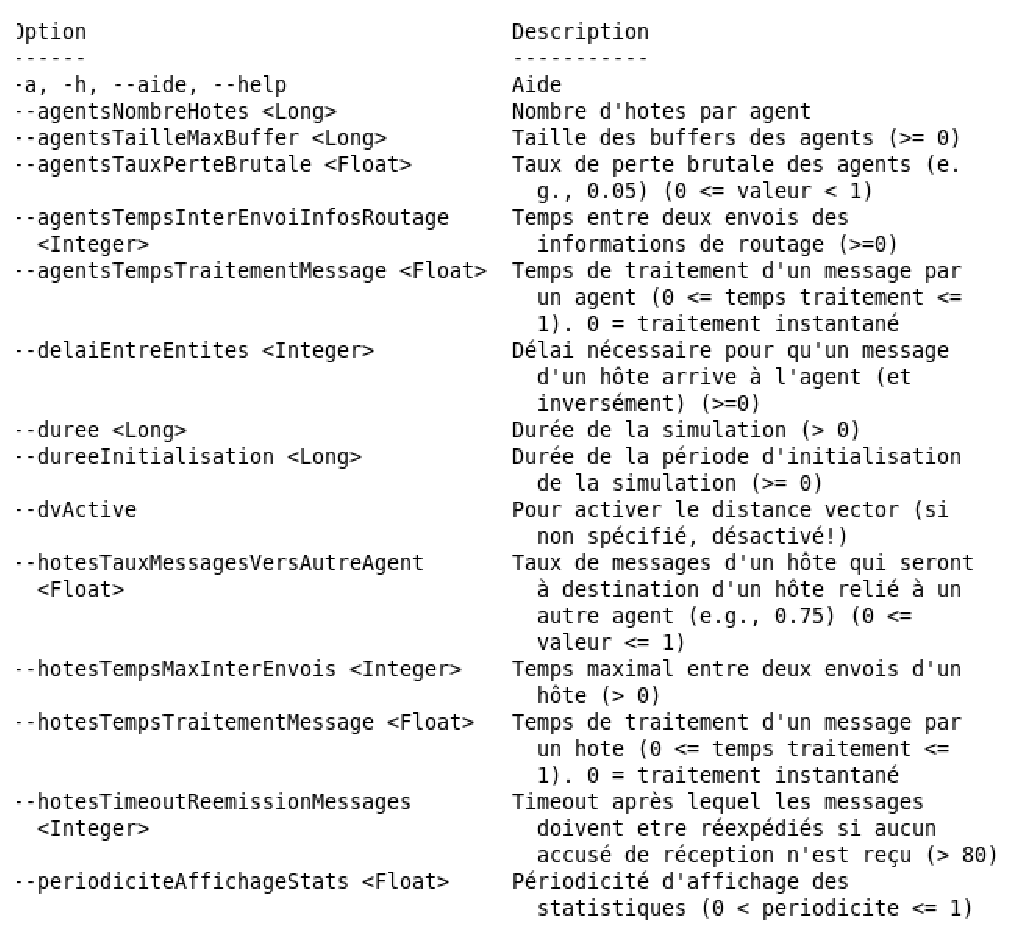
\includegraphics[scale=0.65]{options}
  \caption{Options disponibles}
  \label{fig:options}
\end{figure}

Ensuite pour spécifier les options, on peut par exemple faire: \textbf{java -jar simulation.jar --agentNombreHotes 1000 --duree 5000}.

\subsection{Organisation du code source}
\begin{itemize}
 \item Les sources se trouvent dans le dossier \textbf{src/main/java}
 \item Les fichiers de configuration par défaut se trouvent dans le dossier \textbf{src/main/resources/configuration}
\end{itemize}

Le point d'entrée du programme est la classe \textit{Main} qui se trouve dans \textbf{src/main/java/be/simulation}.

\subsection{Exécution de la simulation}
Lancer le programme exécute directement la simulation. Si aucune option n'est spécifiée en argument au programme, les valeurs par défaut sont utilisées. Les résultats sont affichés à l'écran et sauvegardés dans un fichier de log.

\subsection{Compilation}
La compilation du code requiert l'utilisation de Maven (\url{http://maven.apache.org/}), un outil de build très simple d'utilisation. En étant dans le dossier du projet (au niveau où se trouve le fichier \textbf{pom.xml}), il suffit d'exécuter la commande suivante: \textbf{mvn package}. Une fois terminé, le fichier jar exécutable est disponible dans le dossier \textbf{target/dist}.

Maven est très simple à installer sur la plupart des distributions Linux (e.g., Ubuntu, ...). Sous Windows, il suffit de le télécharger et d'ajouter le dossier bin au path.